\section{Simulations for Stationary Strategies}
\begin{figure}
  \centering
    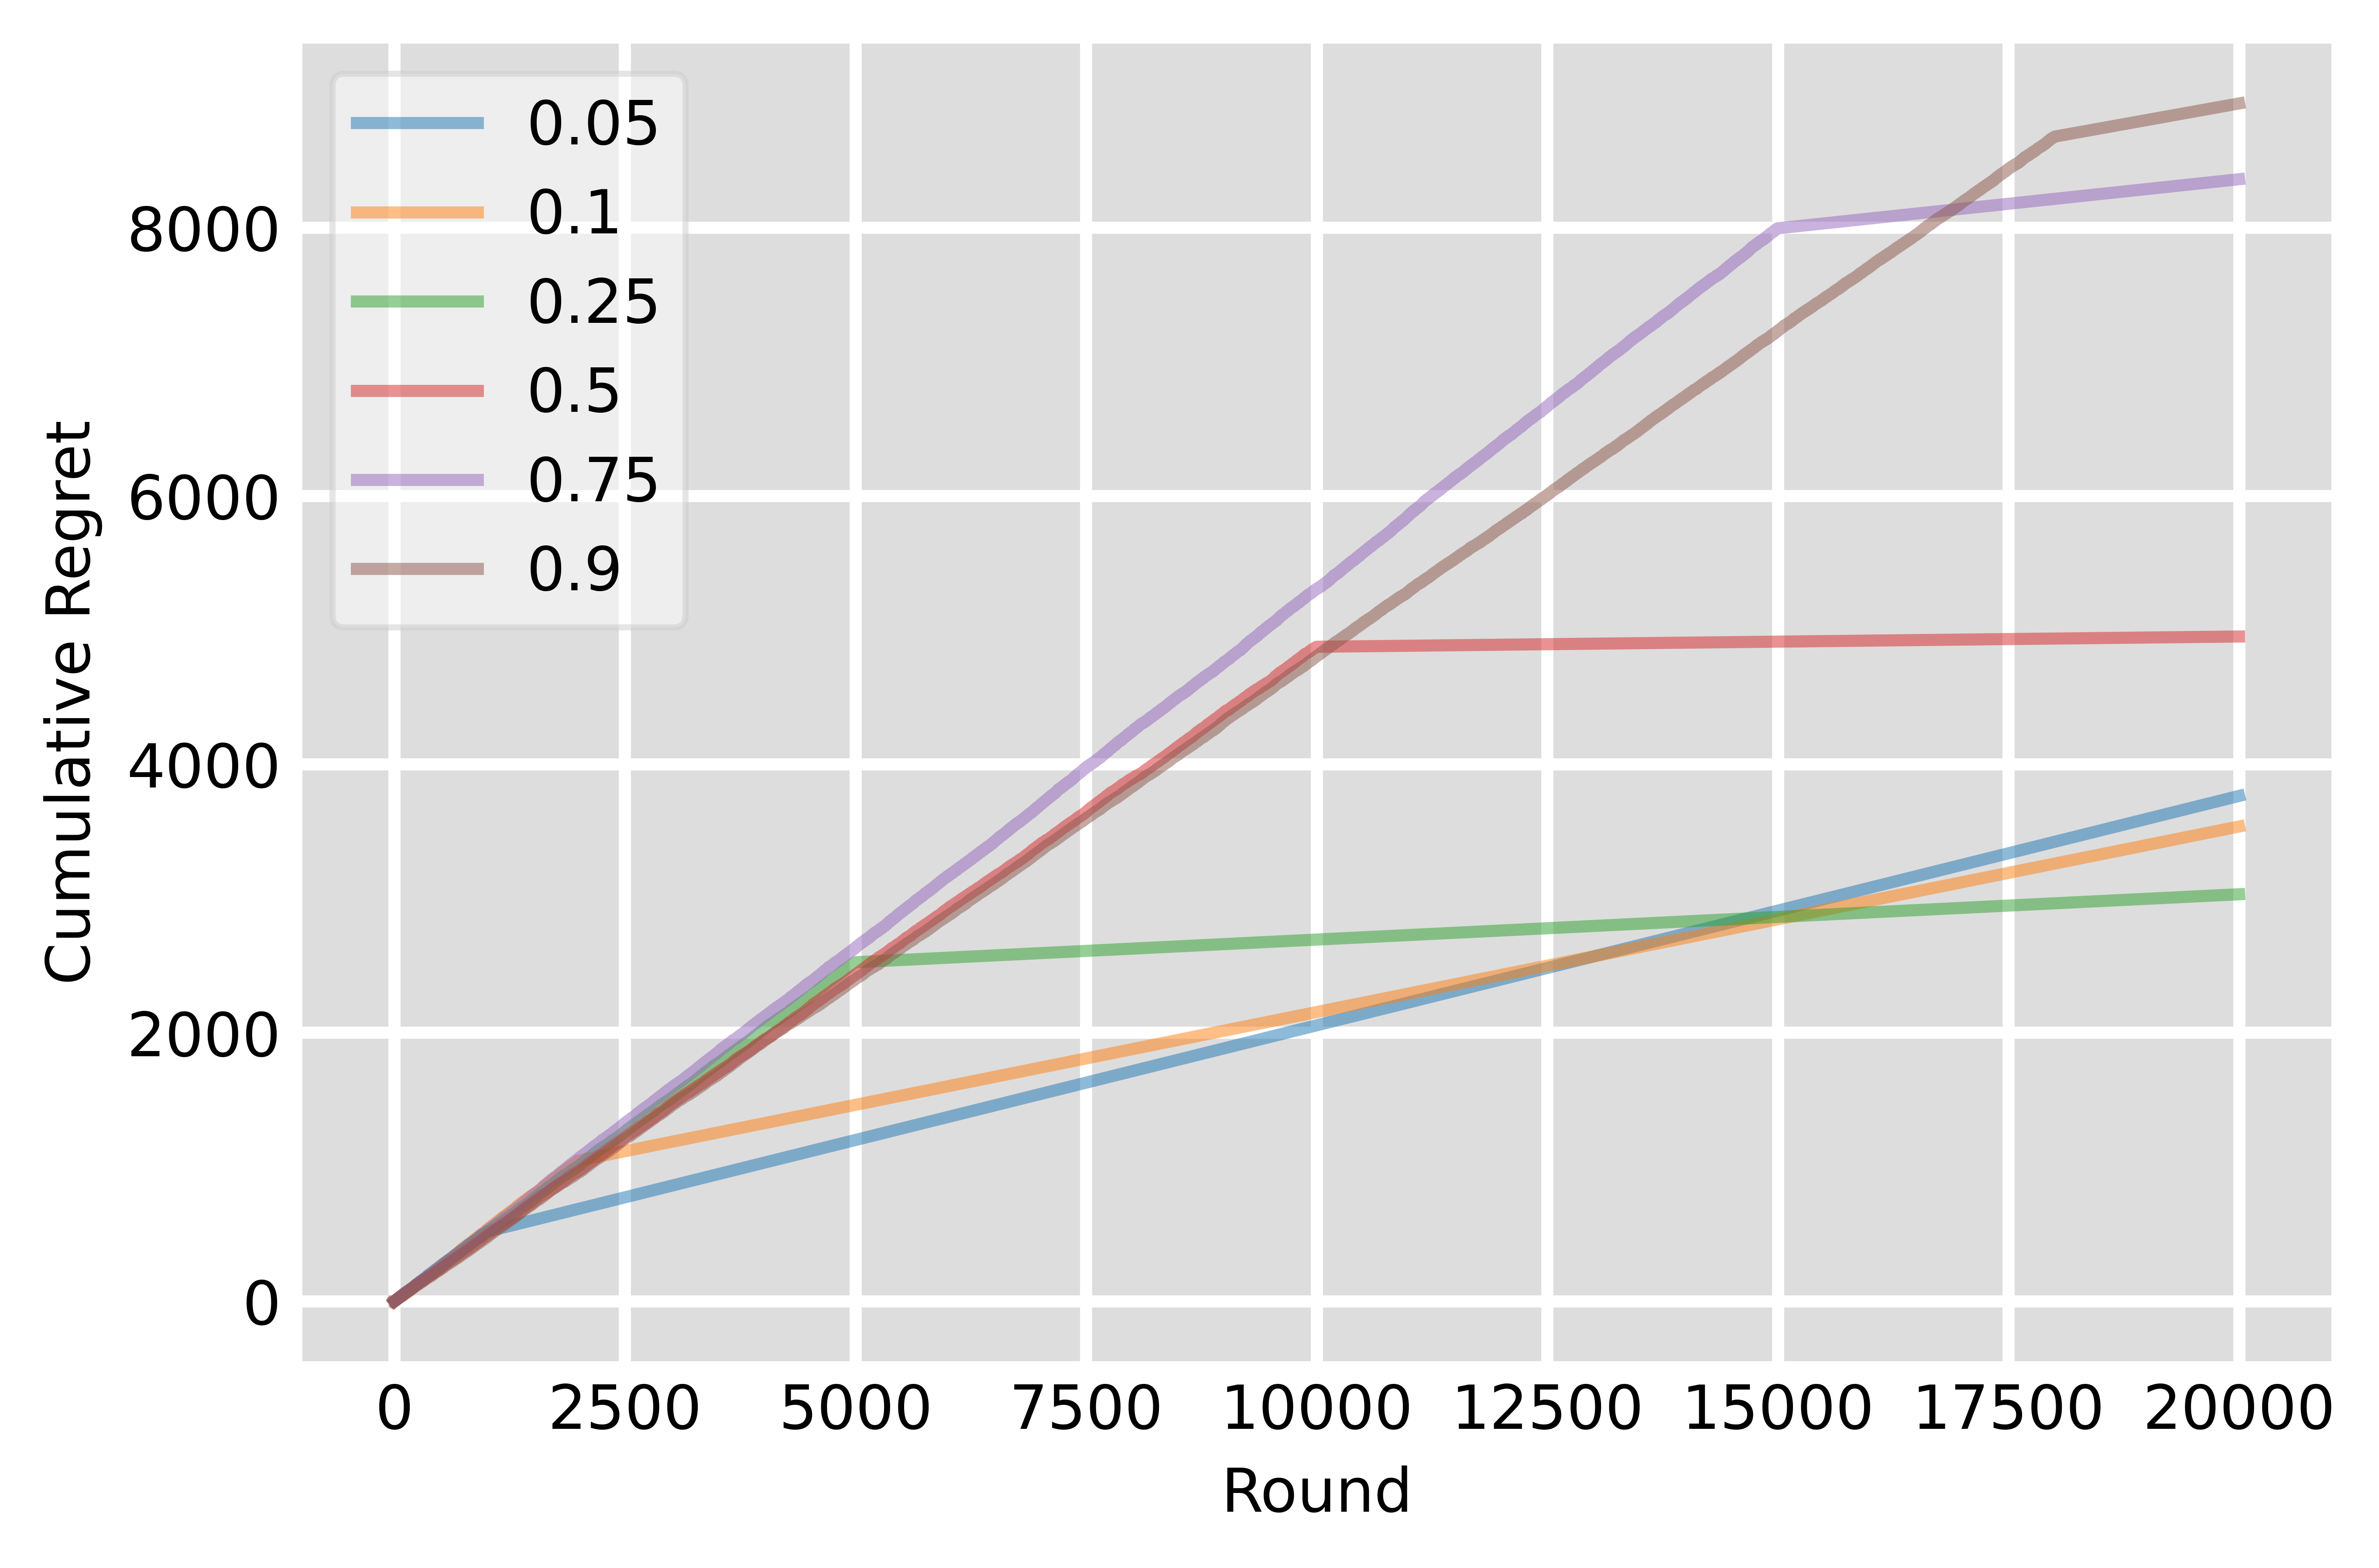
\includegraphics[width=0.9\textwidth]{figures/epsilon_plot.png}
    \caption[Epsilon-first strategy with varying values of epsilon]{Epsilon-first strategy with varying values of epsilon. 100 machines. 20000 rounds per iteration. Average of 50 iterations}
    \label{fig: epsilon}
\end{figure}

\begin{figure}
  \centering
    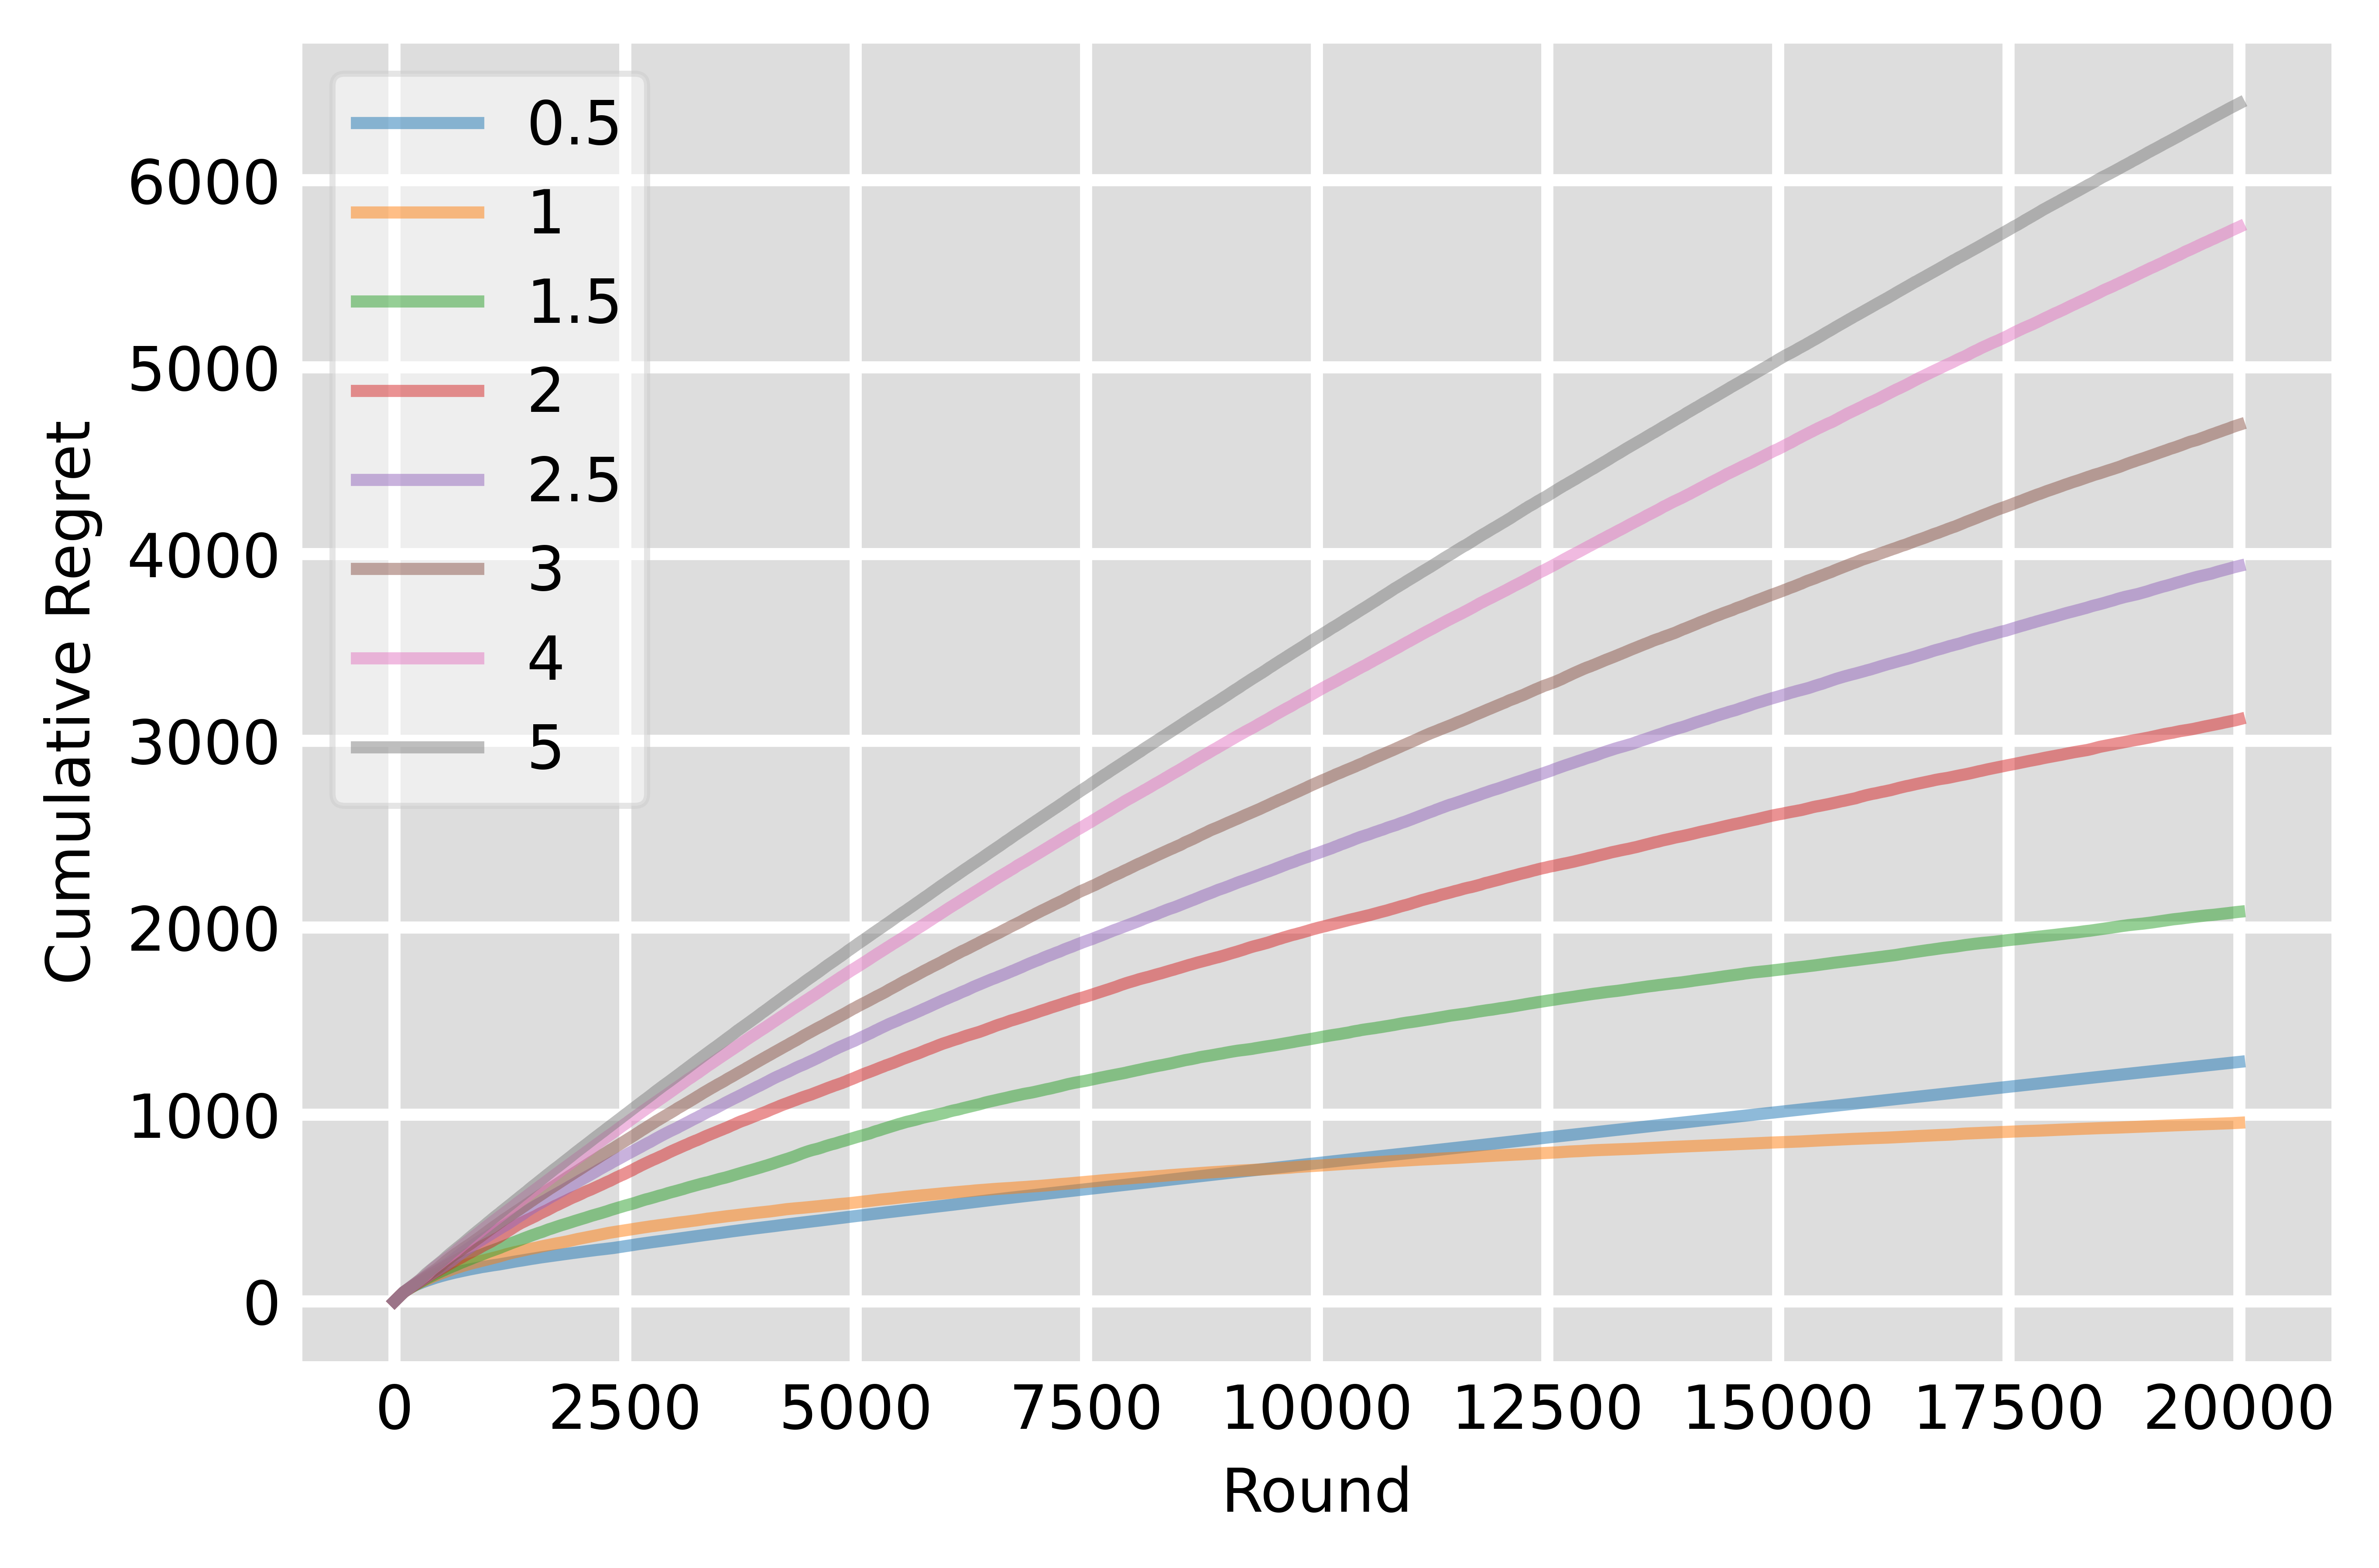
\includegraphics[width=0.9\textwidth]{figures/ucb_plot.png}
    \caption[UCB strategy with varying values of confidence level]{UCB strategy with varying values of confidence level. 100 machines. 20000 rounds per iteration. Average of 50 iterations}
    \label{fig: ucb}
\end{figure}

\begin{figure}
  \centering
    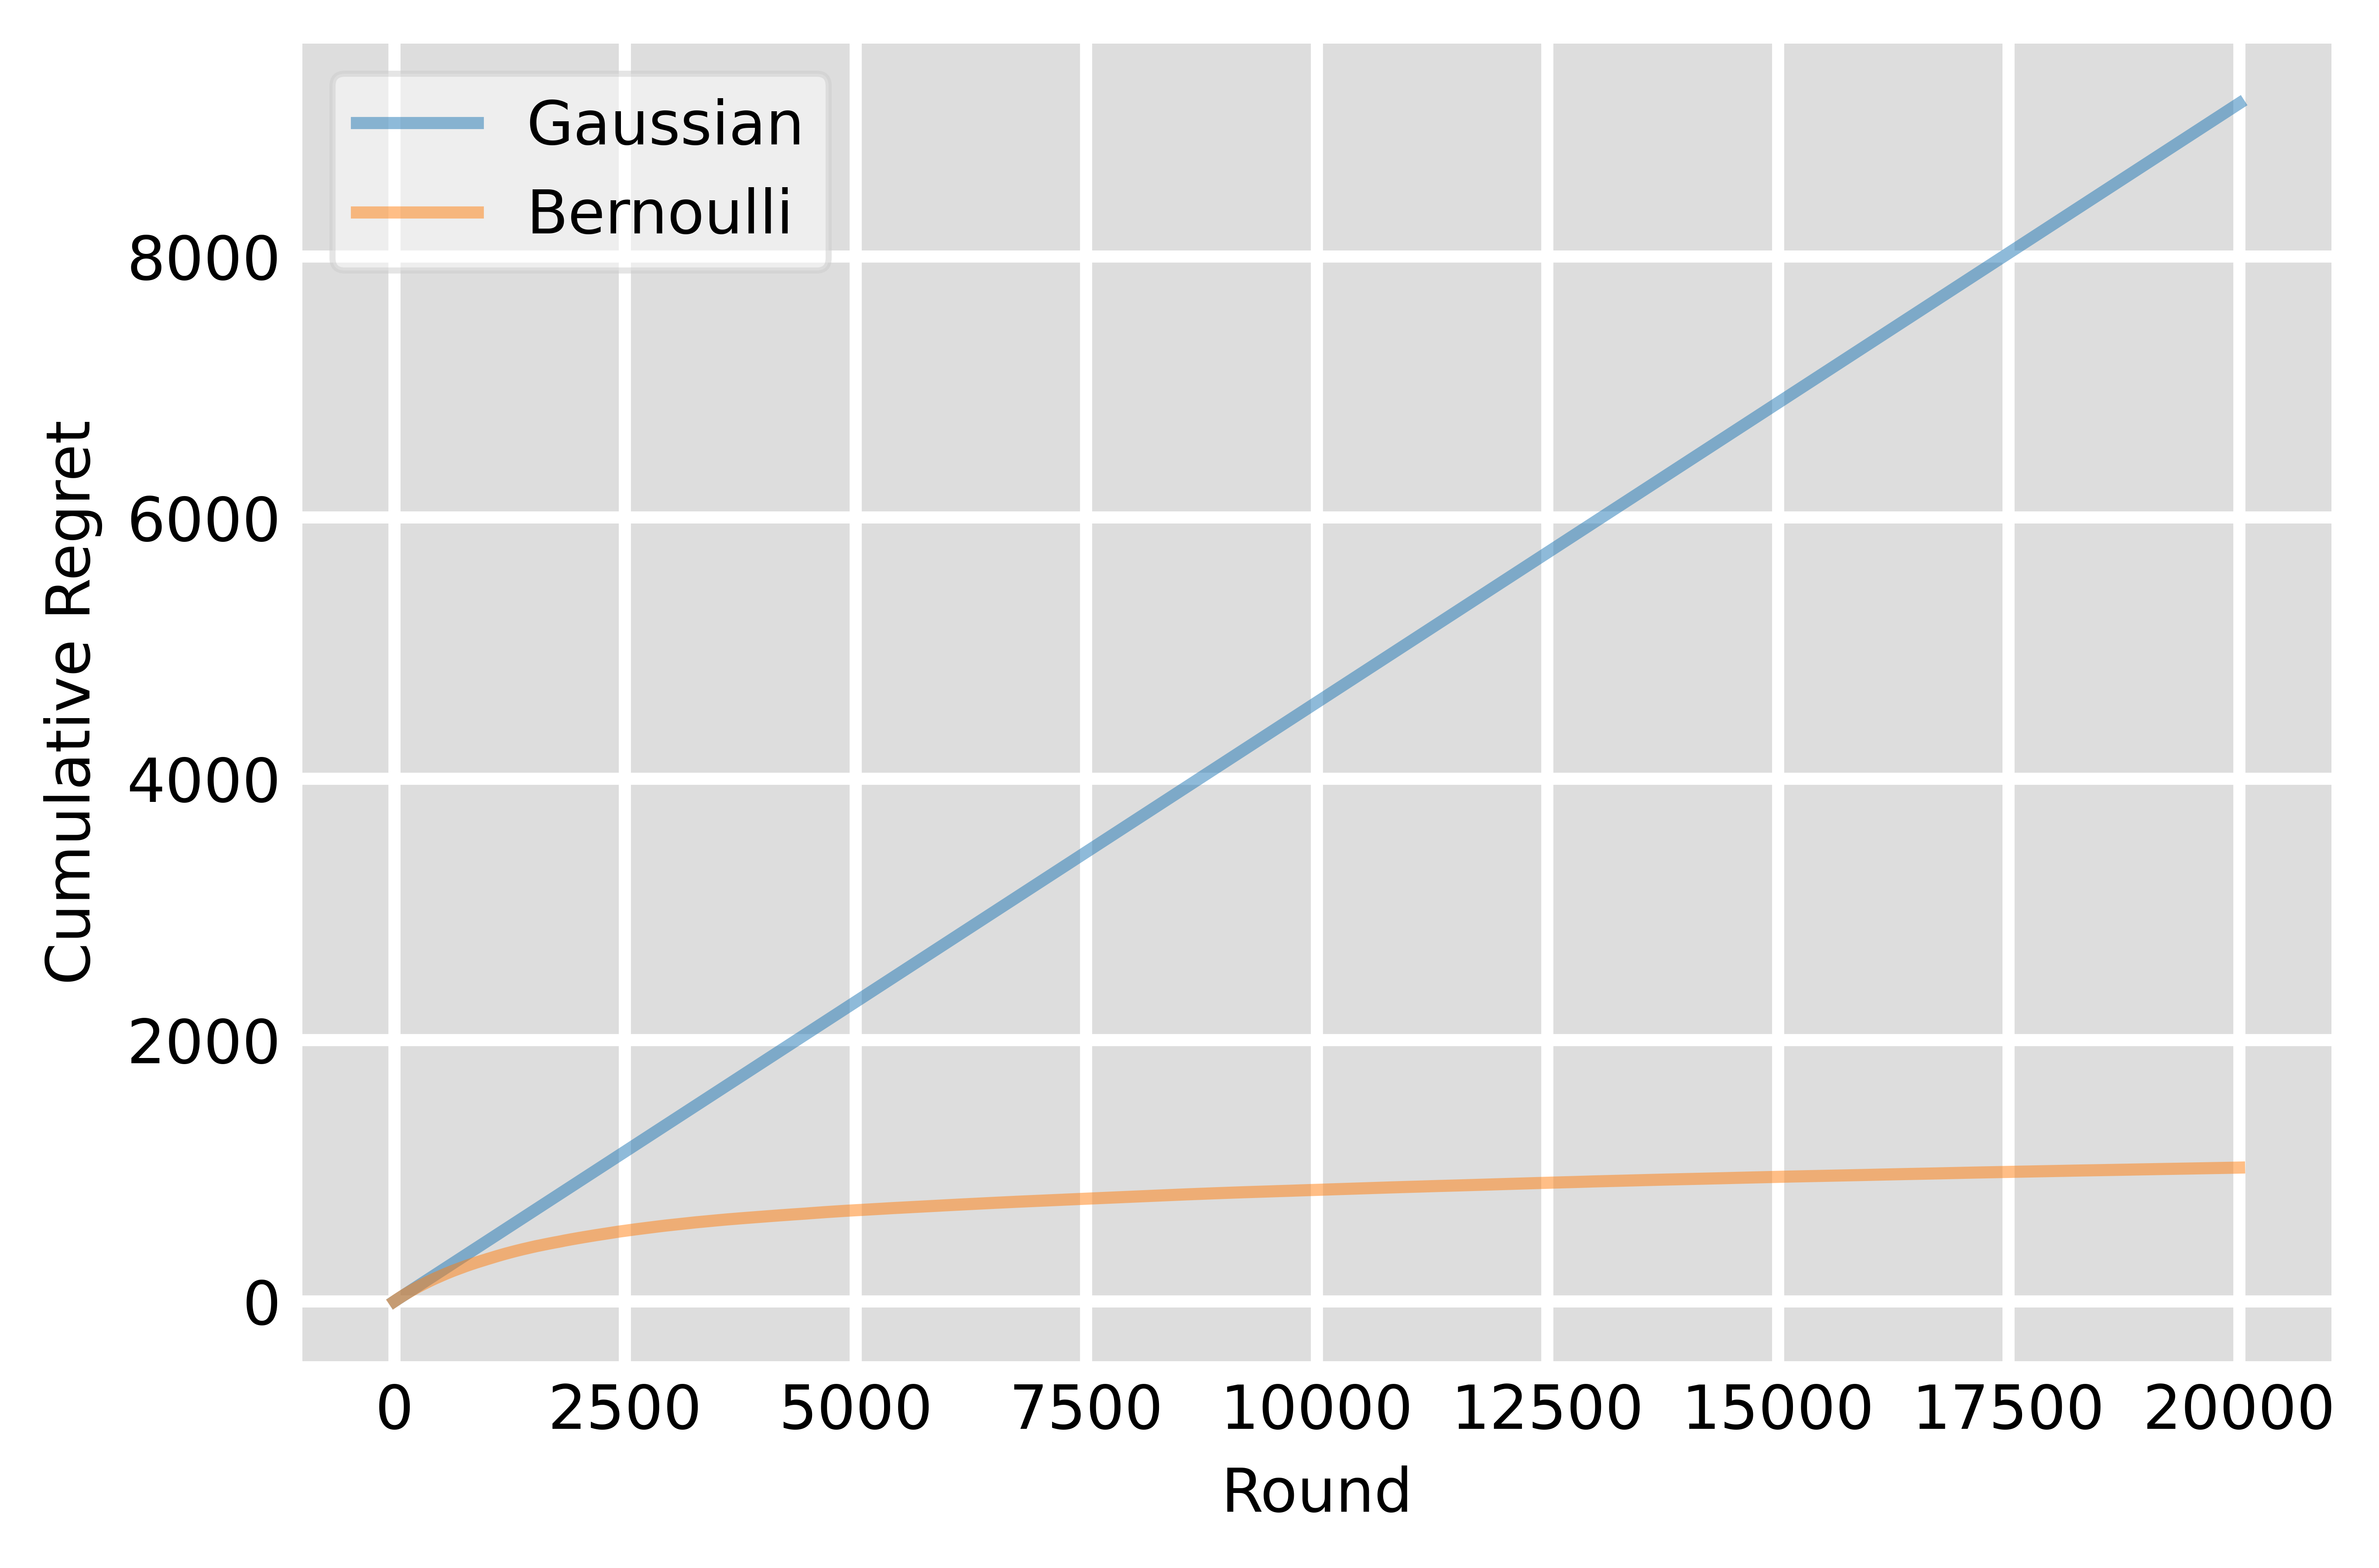
\includegraphics[width=0.9\textwidth]{figures/thompson_plot.png}
    \caption[Thompson strategy with either Bernoulli or Gaussian arms]{Thompson strategy with either Bernoulli or Gaussian arms. 100 machines. 20000 rounds per iteration. Average of 50 iterations}
    \label{fig: thompson}
\end{figure}

\begin{figure}
  \centering
    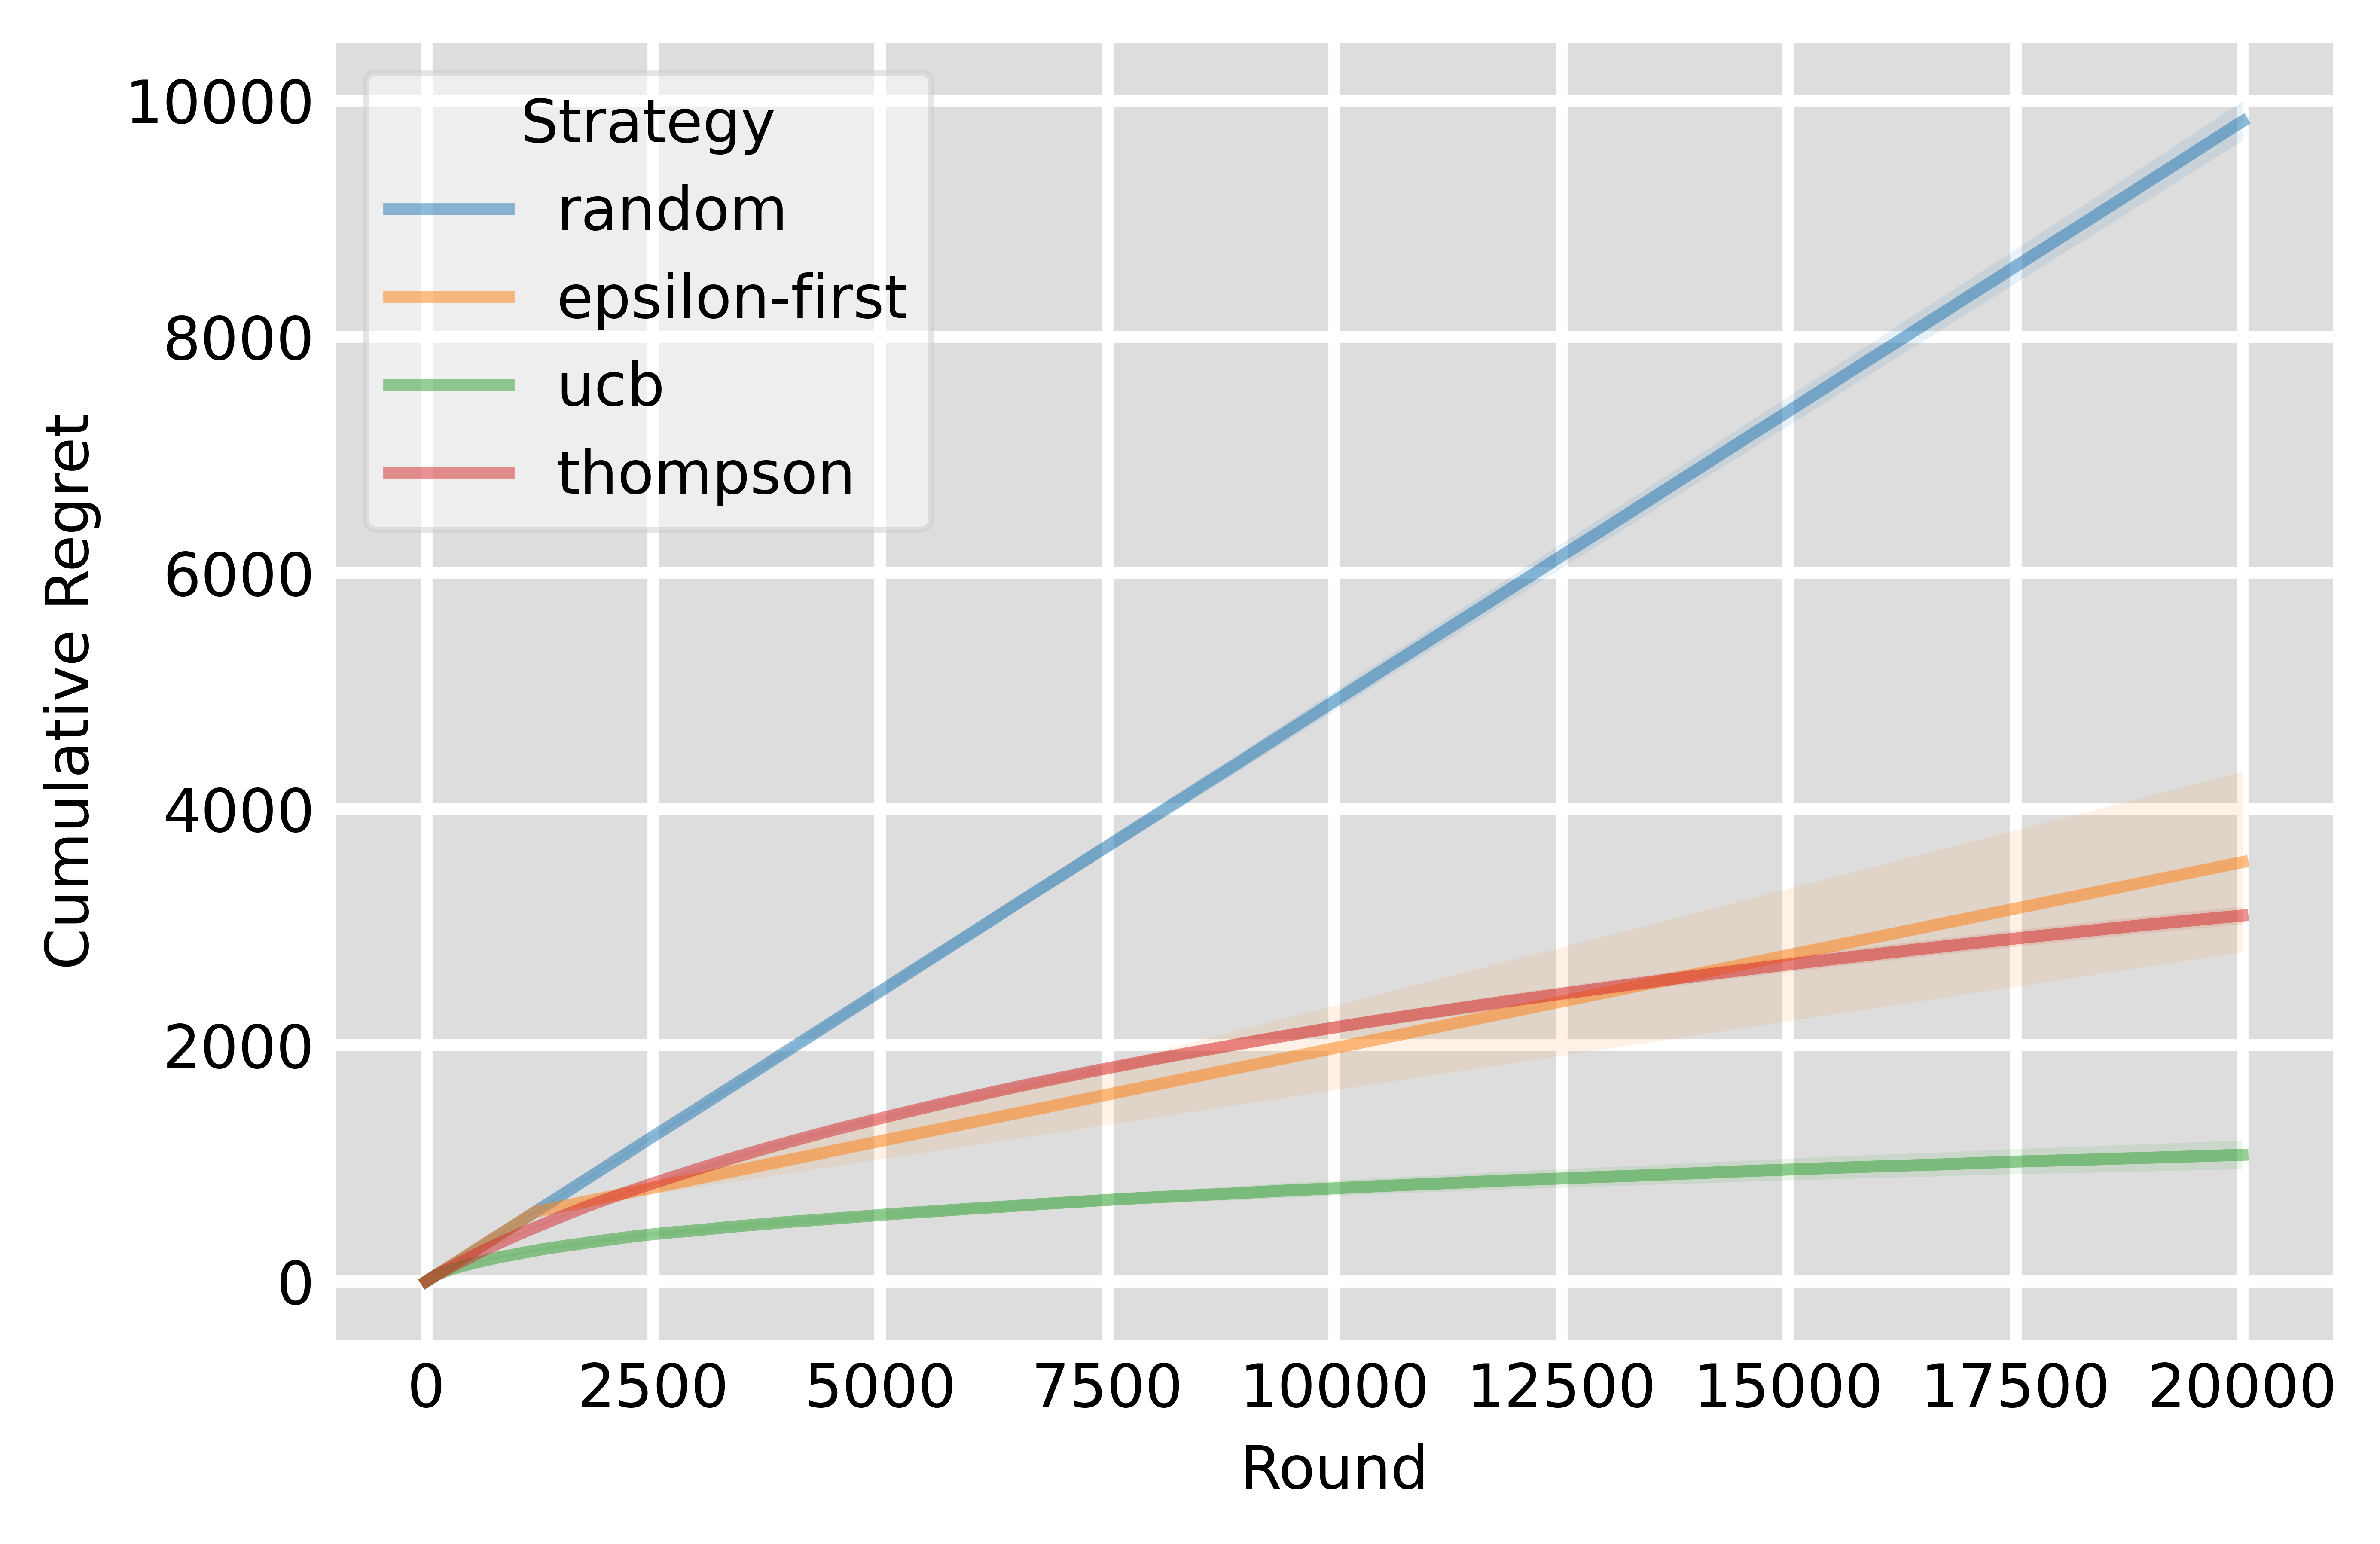
\includegraphics[width=0.9\textwidth]{figures/plot.png}
    \caption[Comparison of Stationary Strategies]{Comparison of Stationary Strategies. Epsilon =0.06, confidence level=1. 100 machines. 20000 rounds per iteration. Average of 50 iterations}
    \label{fig: all1}
\end{figure}

\begin{figure}
  \centering
    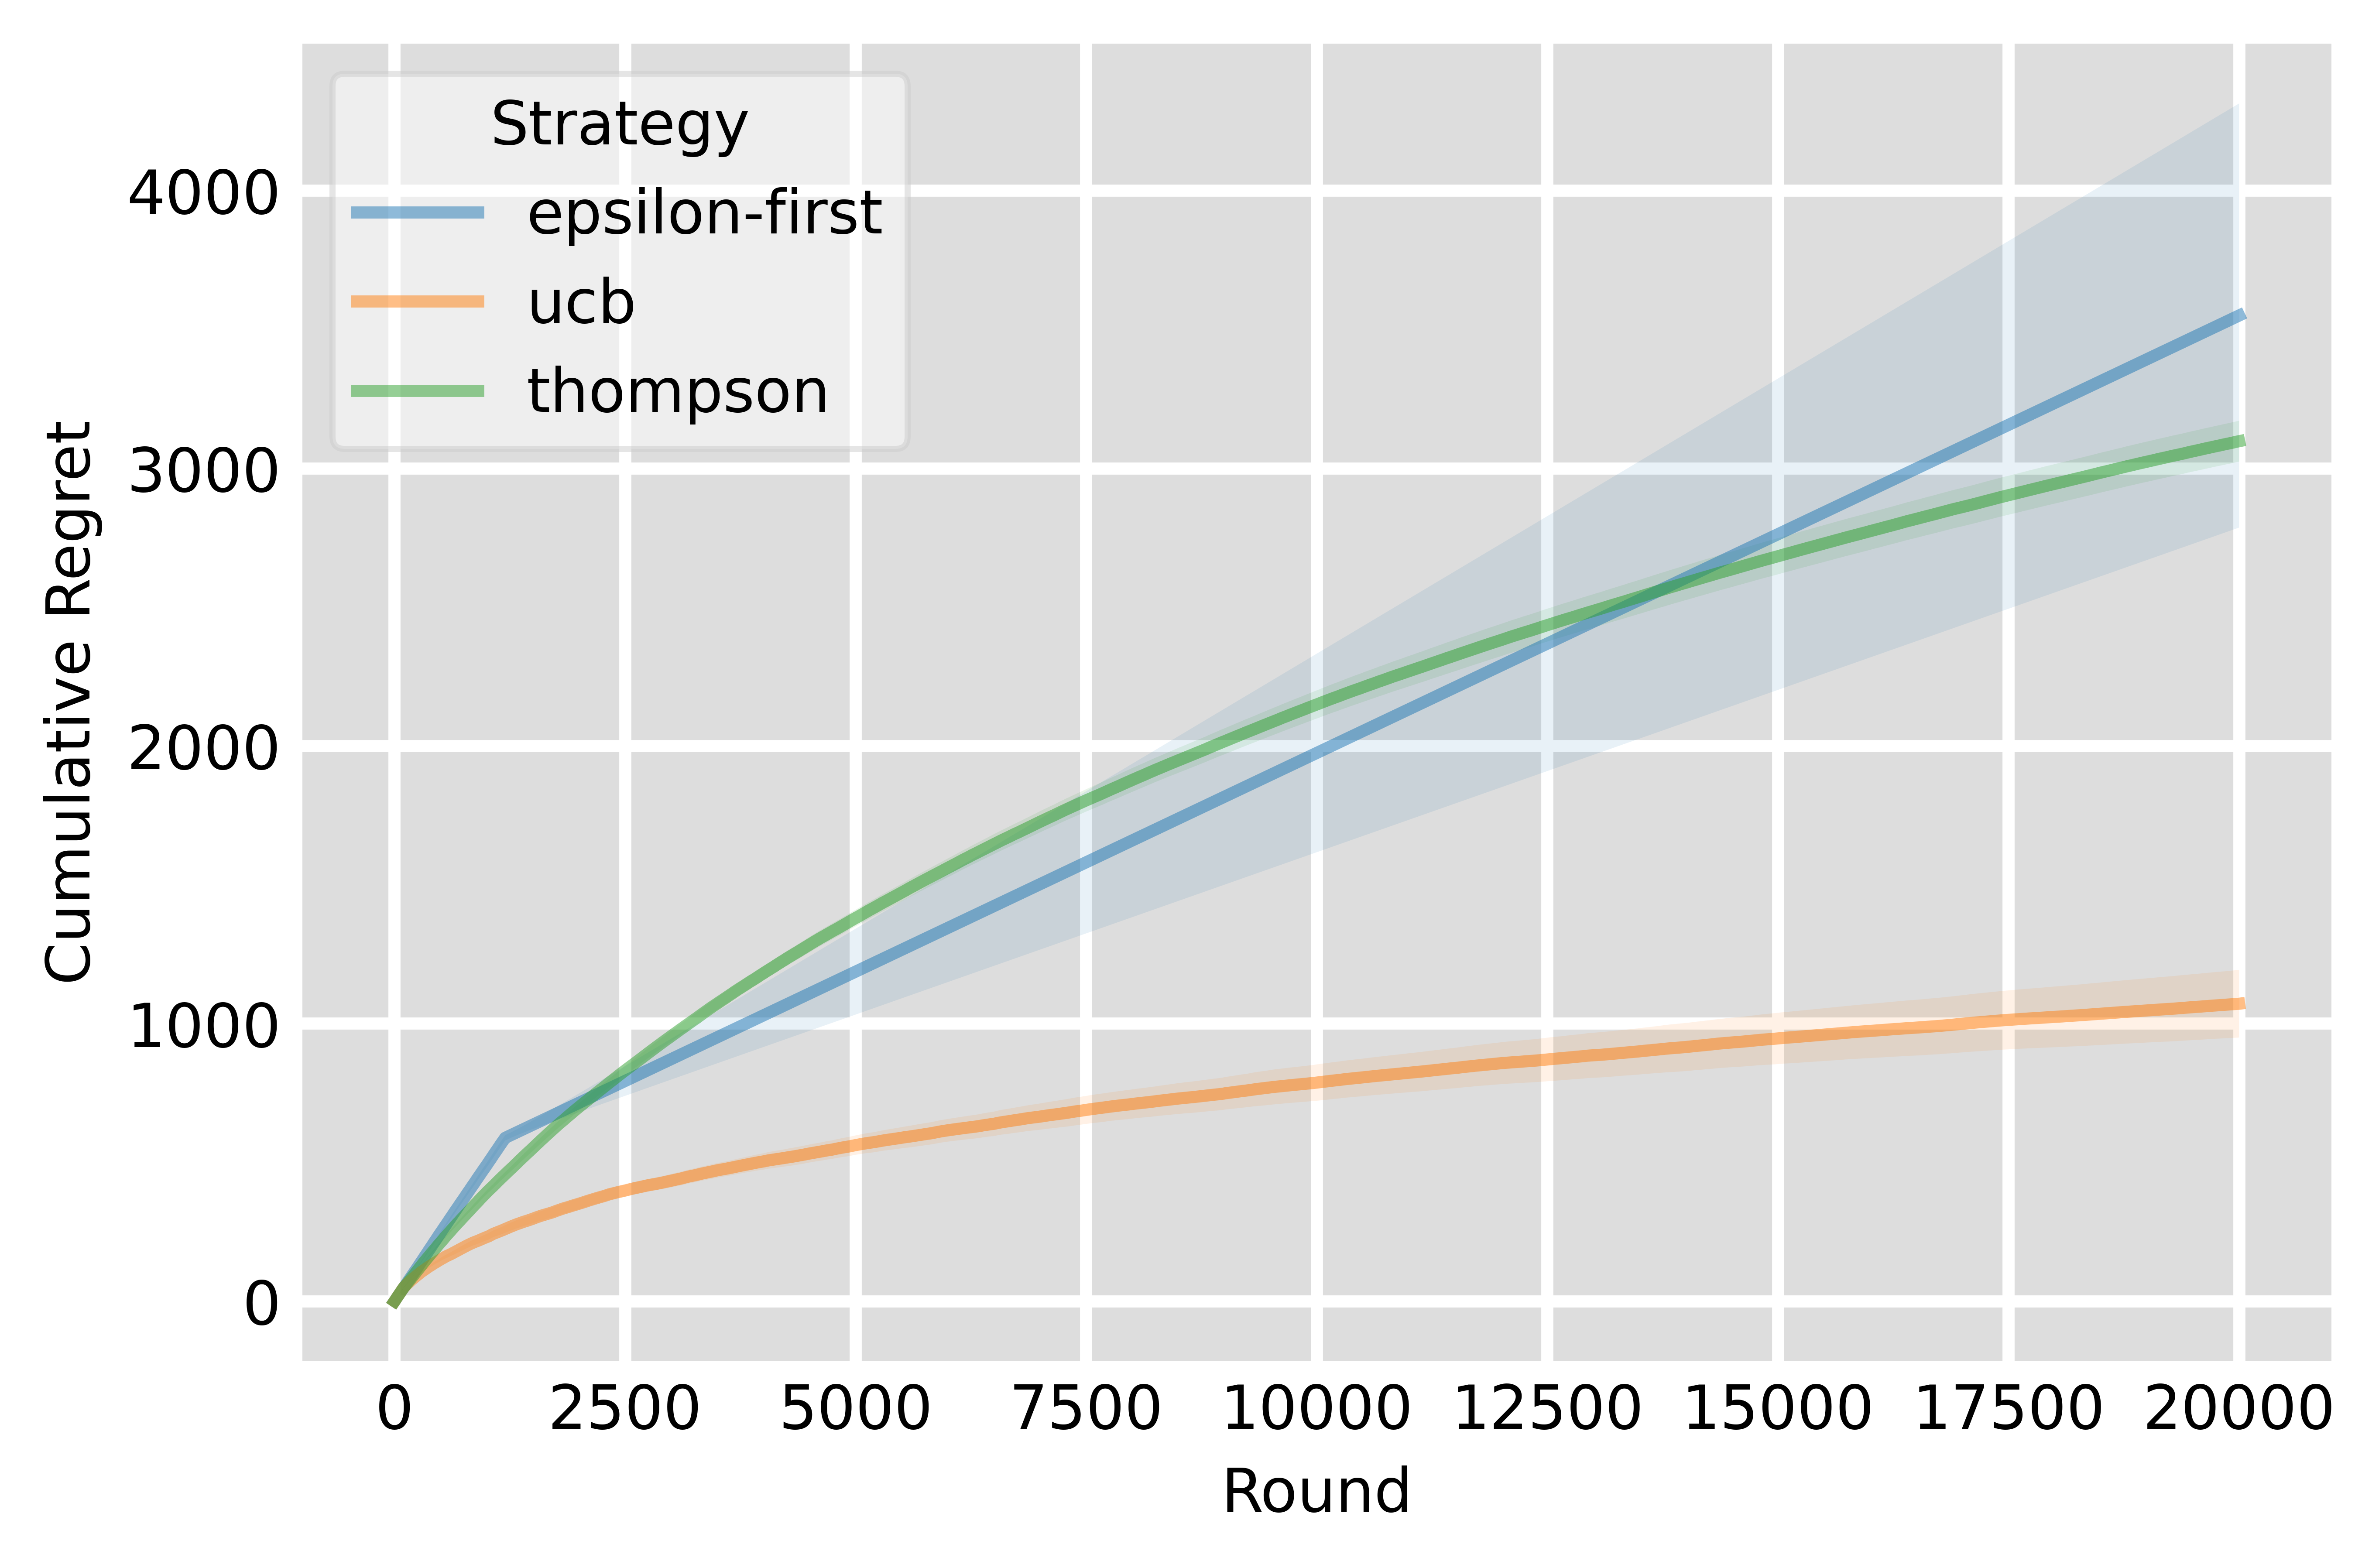
\includegraphics[width=0.9\textwidth]{figures/plot1.png}
    \caption[Comparison of Stationary Strategies without random]{Comparison of Stationary Strategies without random. Epsilon =0.06, confidence level=1. 100 machines. 20000 rounds per iteration. Average of 50 iterations}
    \label{fig: all1}
\end{figure}

\begin{figure}
  \centering
    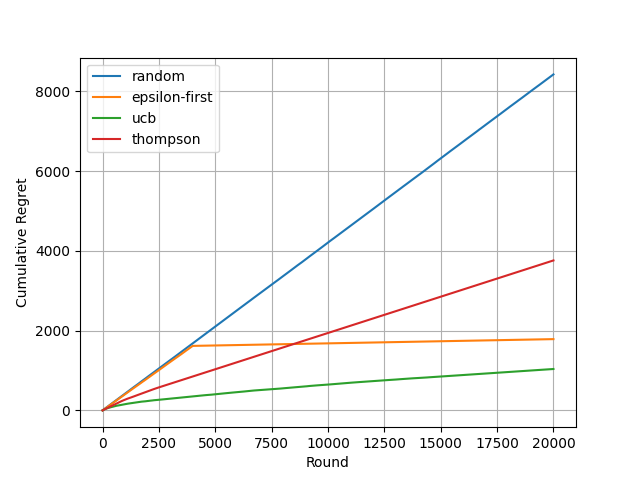
\includegraphics[width=0.9\textwidth]{figures/10machines.png}
    \caption[Comparison of Stationary Strategies]{Comparison of Stationary Strategies. Epsilon =0.2, confidence level=1. 10 machines. 20000 rounds per iteration. 20 iterations}
    \label{fig: all3}
\end{figure}

\begin{figure}
  \centering
    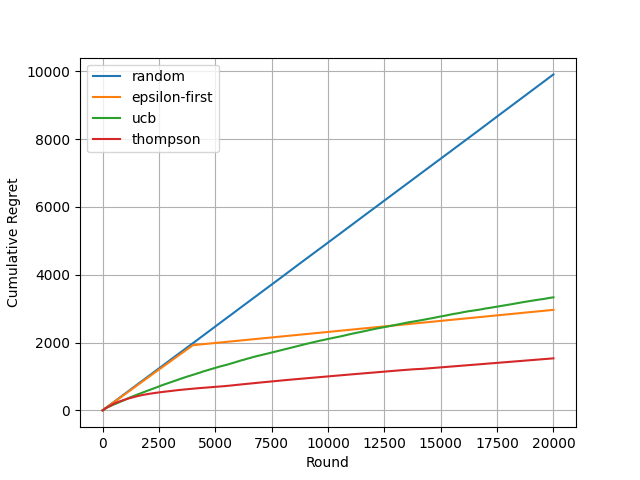
\includegraphics[width=0.9\textwidth]{figures/100machines.png}
    \caption[Comparison of Stationary Strategies]{Comparison of Stationary Strategies. Epsilon =0.2, confidence level=1. 100 machines. 20000 rounds per iteration. 20 iterations}
    \label{fig: all4}
\end{figure}

